This chapter will discuss the process of eliciting and prioritising functional and non-functional requirements for the application. This was not only performed at the start of the project, but, was in fact an iterative process with many new requirements being uncovered during design and implementation stages.
\section{Eliciting of Requirements}
To elicit the requirements of the application user personas were created to represent potential users of the system. These personas were then used to create user stories that would provide a better understanding of what functionality a potential user would want, and why. Requirements were also elicited through brainstorming sessions alone and with the project supervisor.
\subsection{User Personas} \label{personas}
Personas were created to help build a greater understanding of who the potential end-users for the application would be. Each persona described a potential end-user, and their goals and frustrations. This gave a deeper understanding into why a user would want to use the application and what for.
\begin{figure}[!htbp]
    \centering
    \begin{subfigure}[b]{0.45\textwidth}
        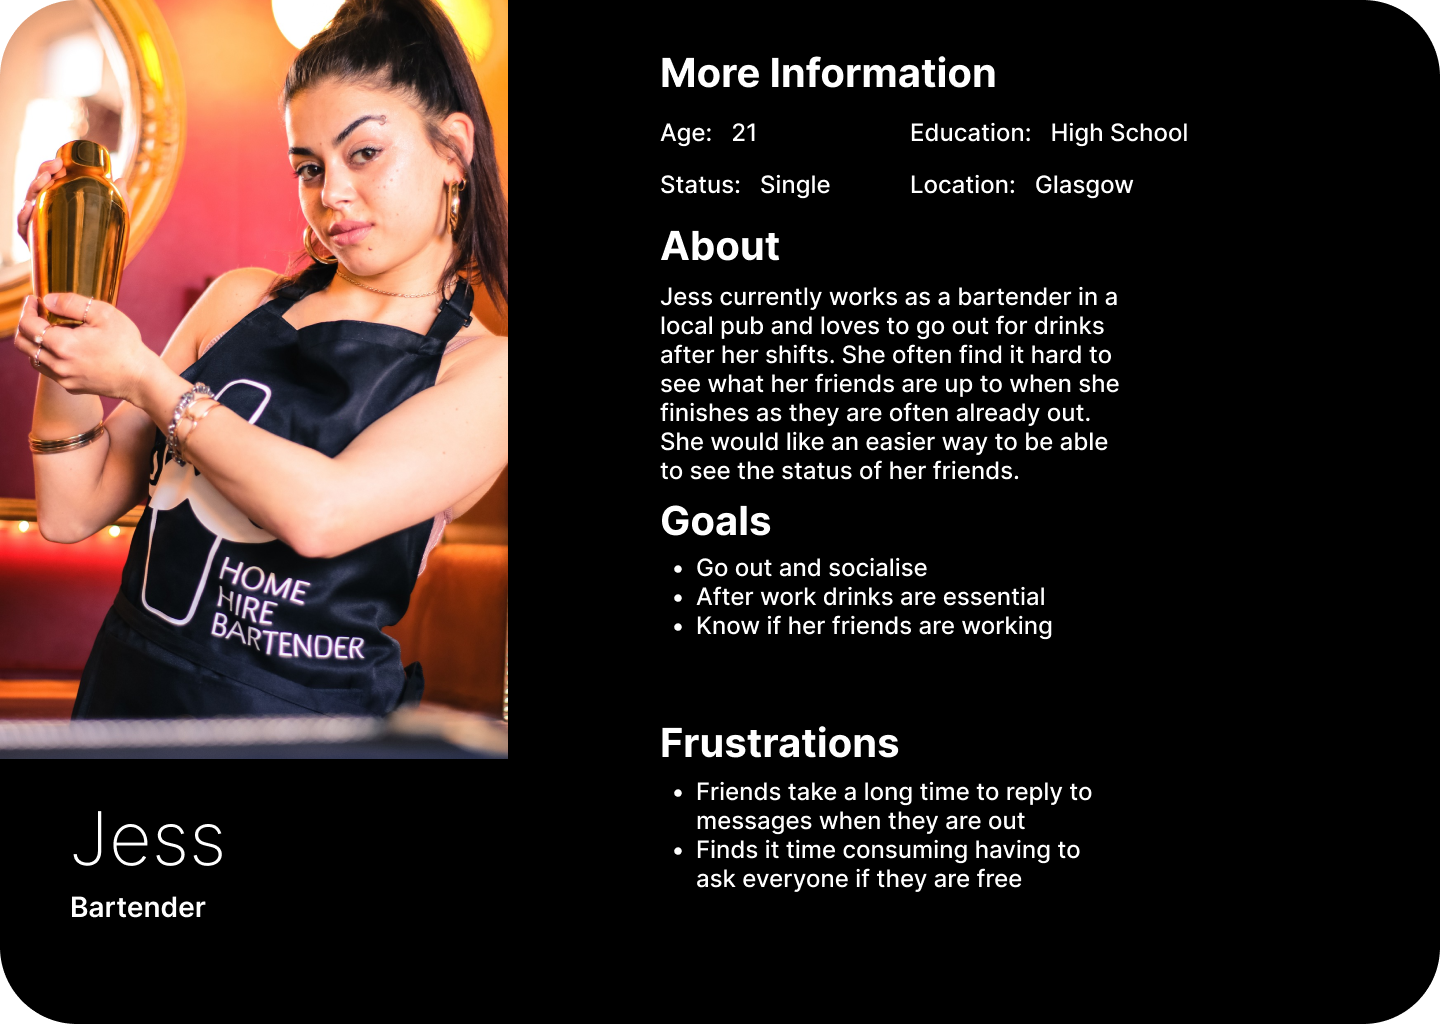
\includegraphics[width=\textwidth]{User_Persona_1.png}
    \end{subfigure}
    \hspace{0.5em}
    \begin{subfigure}[b]{0.45\textwidth}
        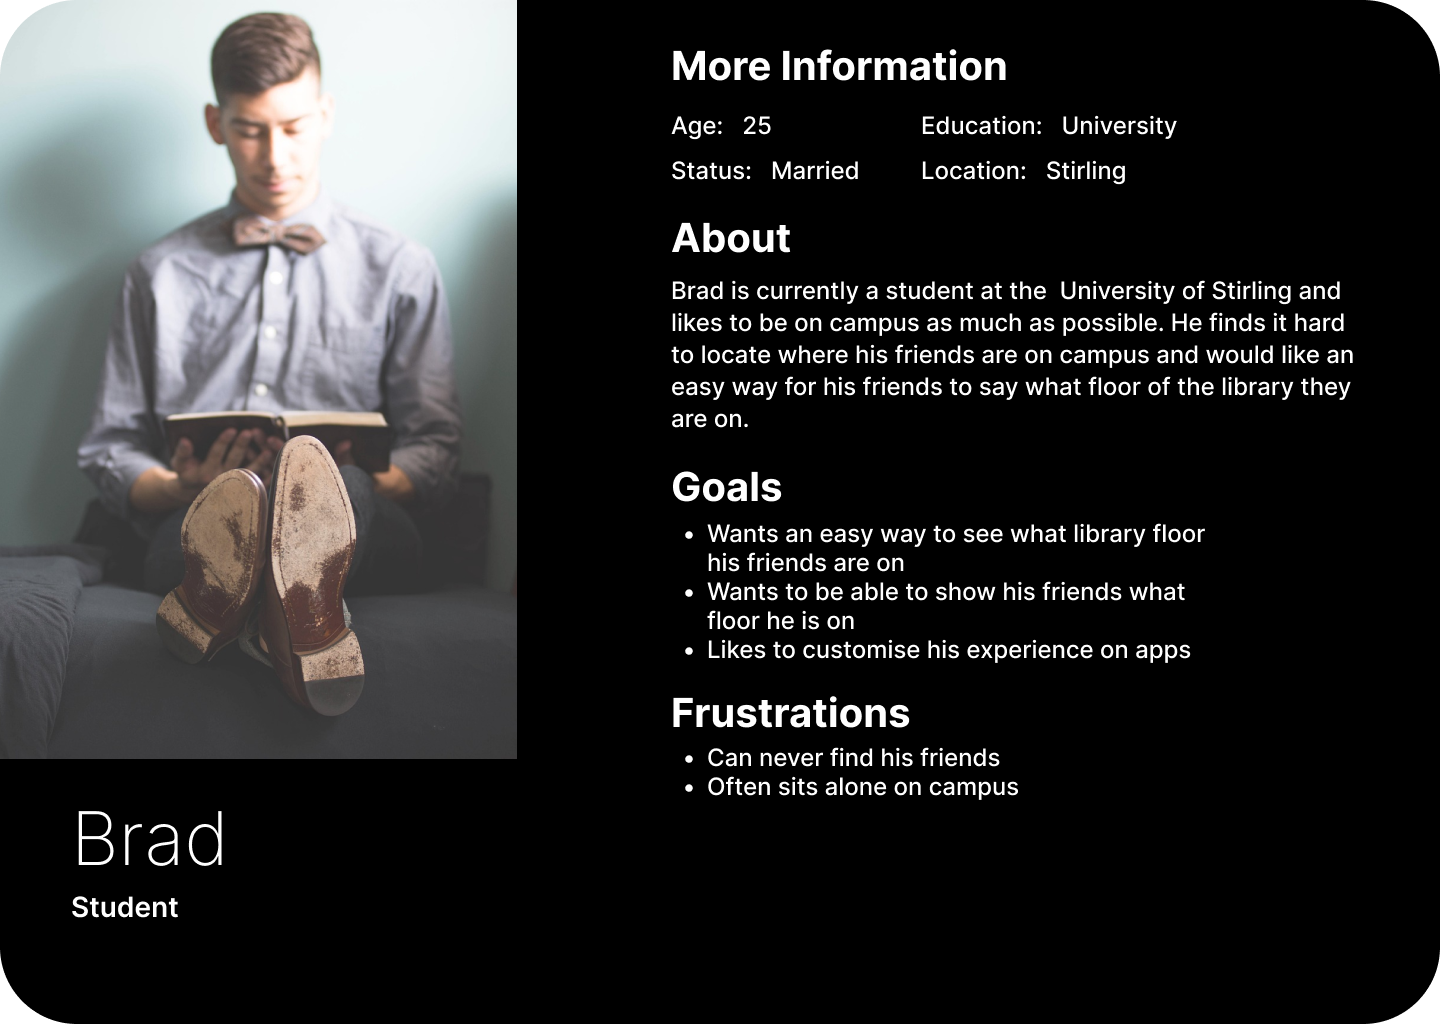
\includegraphics[width=\textwidth]{User_Persona_2.png}
    \end{subfigure}
    \\[0.5ex]
    \begin{subfigure}[b]{0.45\textwidth}
        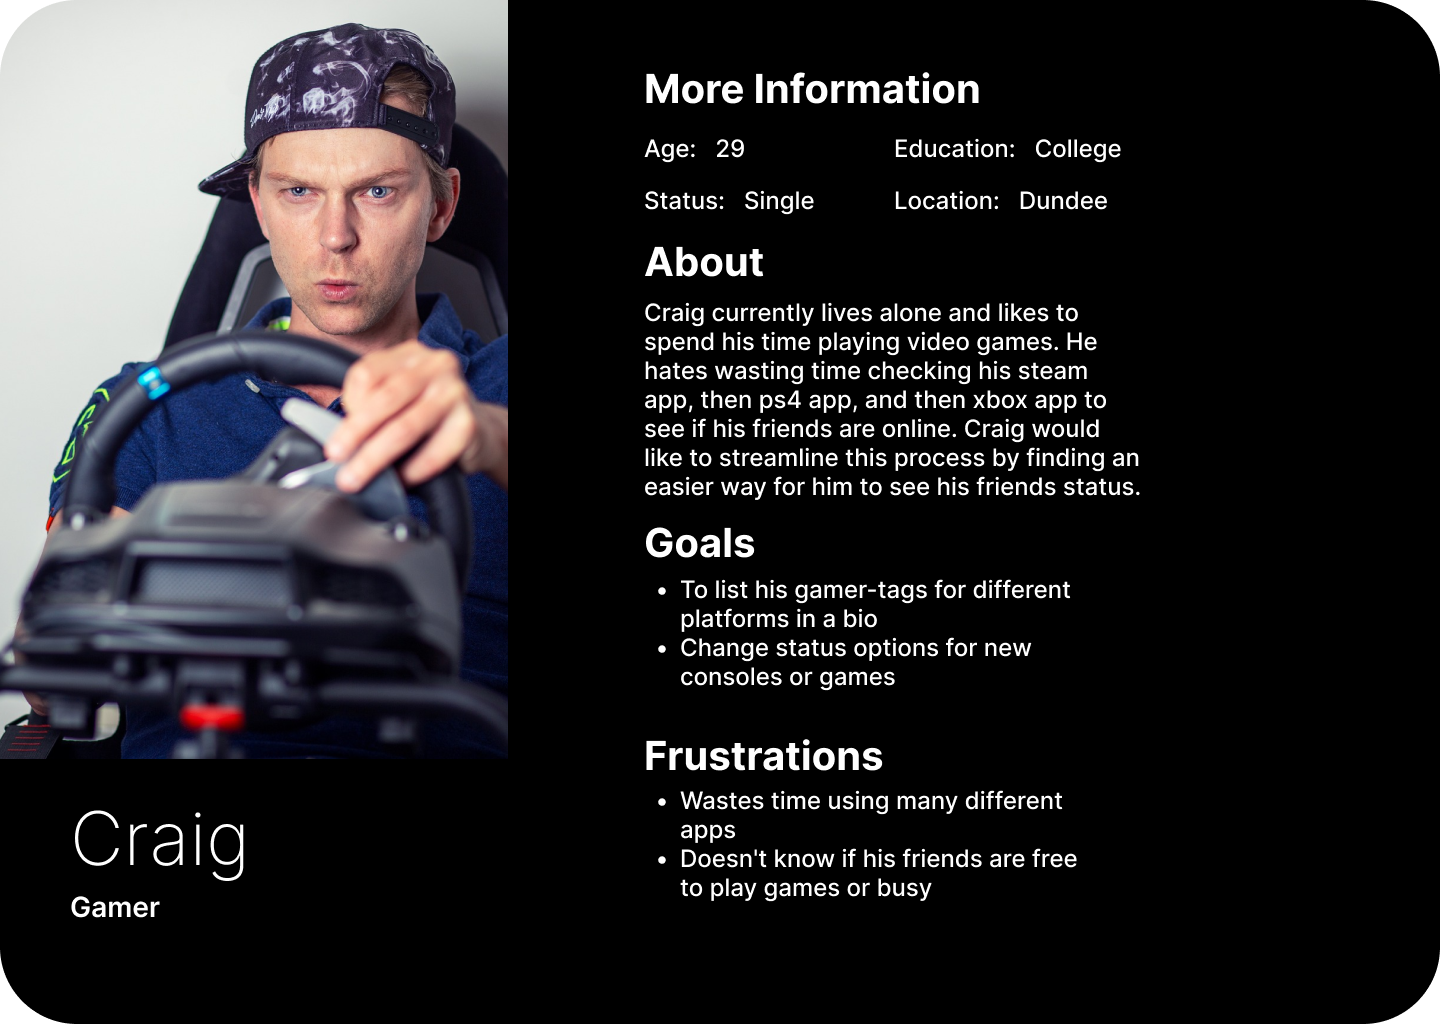
\includegraphics[width=\textwidth]{User_Persona_3.png}
    \end{subfigure}
    \caption{User Personas \textbf{how do i reference this}}
    \label{fig:personas}
\end{figure}
\FloatBarrier
\subsection{User Stories}
User stories were then derived from the personas (see \ref{personas}) to greater understand what a user would use the application to do, and why they want to do it. This process of creating personas to envision potential end-users, then deriving stories, is a common and effective practice for eliciting requirements. 
\begin{figure}[!htbp]
    \centering
    \begin{subfigure}[b]{0.90\textwidth}
        \frame{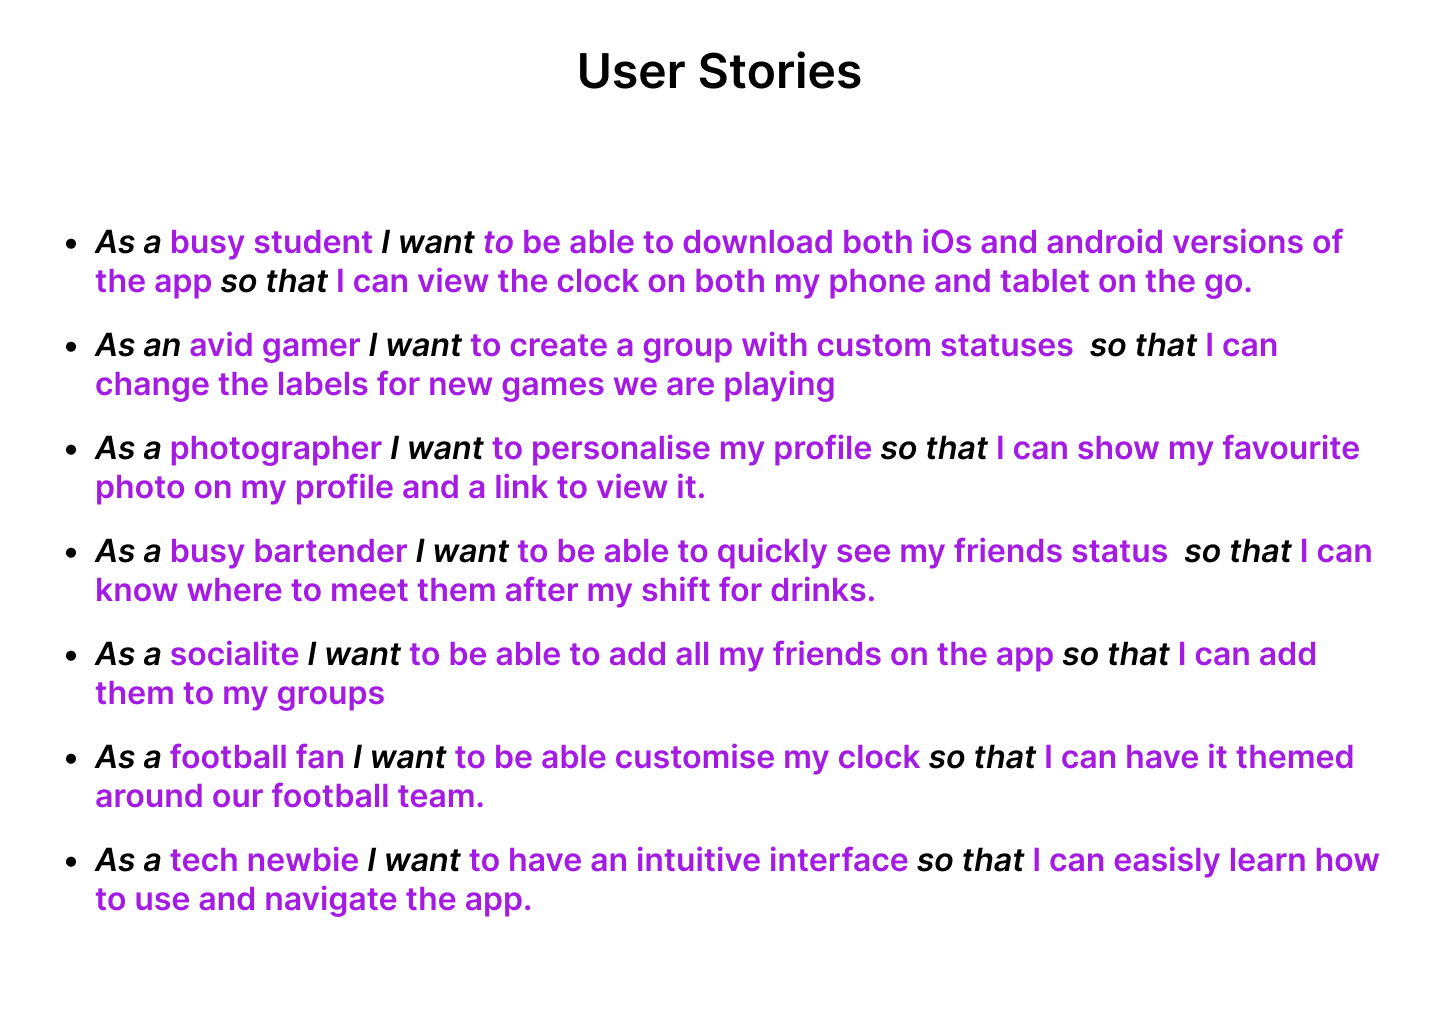
\includegraphics[width=\textwidth]{User_Stories.png}}
    \end{subfigure}
    \caption{User Stories \textbf{how do i reference this}}
    \label{fig:stories}
\end{figure}
\FloatBarrier
\subsection{Brainstorming}
Further requirements were also elicited through brainstorming with the project supervisor throughout the project. Weekly discussions concerning what new features could be implemented, and how potential users could possibly interact with the application helped to further elicit requirements.
\section{Requirement Prioritisation}
Now that the requirements of the app were clearer the next step was to use a prioritisation technique. MoSCoW prioritization \cite{moscow} was used to categorise the requirements into Must Have, Should Have, Could Have, and Wont Have.
\begin{itemize}
    \item \textbf{Must Have (MH)} \par
    Requirements labeled as must have are of the highest priority and are the main requirements that need to be fulfilled. 
    \item \textbf{Should Have (SH)} \par
    Requirements labeled as should have are not essential to the application but they should be fulfilled. These are the second highest priority requirements. 
    \item \textbf{Could Have (CH)} \par
    Requirements labeled as could have would be nice to be fulfilled but are not needed and should not be prioritised. These are the third highest priority requirements. 
    \item \textbf{Wont Have (WH)} \par
    Requirements labeled as wont have are requirements that could be met in further development but are not a priority to be fulfilled at present. These are the lowest priority requirements. 
\end{itemize}
The priority of requirements could change throughout the project due to a change of vision, increased difficulty, or for many other reasons. The requirements are shown in \ref{functional} and \ref{non-functional} in their priority at the end of the project.
\section{Functional Requirements} \label{functional}
\textbf{DO I NEED TO REF FB IOS ANDROID ETC}\par
These requirements are functional, and describe the features that the application should have and what the application should do. 
\begin{enumerate}
    \item \textbf{[MH] The application should be available on both Android and iOS} \par
    This is essential that the application can support both mobile operating systems so that any user can download the application.
    \item \textbf{[MH] The application should utilise Firebase as a back-end} \par
    This is essential that the application has a back-end to store all the data for the application and users. Firebase allows the storage of data in their real time database, and images in storage. Firebase allows the app to have synced data in real time which is a great feature.
    \item \textbf{[MH] The application should display the status of friends on a graphical clock face} \par
    This is the main feature of the application and is essential to the completion of the project.
    \item \textbf{[MH] The application should have a home page displaying the users groups} \par
    This is important as users should be greeted with a display of all their groups so they can easily and efficiently navigate to them.
    \item \textbf{[SH] The application should have the functionality to create a group with your friends} \par
    This is a major feature of the app so that users can be in groups with their friends.
    \item \textbf{[SH] The application should have the functionality to customize the clock} \par
    Different groups of friends may use the clock for different purposes as seen in the user personas (see \ref{personas}), so the ability to change the statuses on the clock is very important. If all users had the same coloured hand this would create difficulties with identifying what user belongs to what hand. Giving the user the ability too change hand colour not only addresses this usability concern, but adds to the personalised experience for that user. The ability to customize the clock face also adds to the personalized experience.
    \item \textbf{[SH] The application should have the functionality to allow customization of the users profile } \par
    Users should be able to change their username, bio, and profile picture for their account. This adds to the personalized experience of the application.
    \item \textbf{[SH] The application should have a friends system } \par
    Users should be able to request to be friends with a user to then allow them to be added to a group.
    \item \textbf{[SH] The application should allow users to have multiple groups } \par
    Most people will have multiple friend groups all with different interests and members. Therefore, users should be able to create groups for these different friends and interests 
    \item \textbf{[SH] The application should have authentication for users } \par
    This ensures that users are validated before they can perform certain operations.
    \item \textbf{[CH] The application should have push notifications } \par
    This was initially added as a could have requirement but was moved to must have as their was a change in the vision of the app that didn't include notifications.
    \item \textbf{[WH] The application should have integration with real world location } \par
    This feature could be implemented at a later date with users having the option to have their GPS location made visible to friends.
    \item \textbf{[WH] The application should have animations } \par
    This is a feature that was briefly explored at the end of implementation but discarded as the to implement it would require a rework of the clock functionality. It was decided that this could be potentially added in a future iteration but was not essential to the application.
\end{enumerate}
\section{Non-Functional Requirements} \label{non-functional}
These requirements are non functional, and address the usability of the application and specific properties it should have, not specific system behaviour. 
\begin{enumerate}
    \item \textbf{[MH] The application should have an intuitive navigation system }\par
    Users should be able to easily navigate throughout the app without any prior knowledge or instruction.
    \item \textbf{[MH] The application should have a visually pleasing UI throughout the app }\par
    Users should want to load up the app and without a user interface that is pleasing, many users would not use the application. This also is a usability concern as congested and badly designed UI can create many issues for the user.
    \item \textbf{[MH] The application should have a high level of accessibility }\par
    There should be no obvious accessibility issues. Although there is not enough time or resources available to ensure full accessibility for impairments such as sight, a good effort shall be made.
    \item \textbf{[SH] The application should have fast loading times }\par
    The application should not take a long time to load. Long loading times can make users leave the application and get very frustrated when using.
    \item \textbf{[WH] The application should have integration with dark mode }\par
    In the future a different colour scheme could be used for when dark mode is activated on the users device. However, this was not essential to the operation of the application so was not implemented. 
\end{enumerate}
\section{Summary}